\chapter{Cơ sở lý thuyết} \label{chap:theory}
    \section{Cấu tạo Quadcopter}
    	\subsection{Bộ khung}
Các phần chính của bộ khung Quadcopter được tóm tắt trong bảng sau:
\begin{tabular}{|c|c|c|}
\hline 
Số lượng & Tên & Kích thước \\ 
\hline 
1 & Bộ điều khiển trung tâm & 155mm \\ 
\hline 
4 & Khung & 330mm \\ 
\hline 
2 & Càng hạ/cất cánh & 220mm \\ 
\hline 
\end{tabular}
\begin{itemize}

\item Bộ điều khiển trung tậm được tạo từ hai tấm vật liệu carbon gắn chặt với nhau và khung Quadcopter. Bộ điều khiển sử dụng chương trình Adrupilot để kiểm soát bay. Ngoài ra bên trong bộ điều khiển còn chứa dây nguồn,… Pin Li-polymer được đặt ở dưới cùng bộ điều khiển để tạo sự ổn định khi bay. 

\item Khung Quadcopter được tạo thành từ các thanh Carbon rỗng. Các thanh này được gắn chặt với bộ điều khiển thông qua các miếng cao su để giảm chấn khi động cơ hoạt động. Bốn thanh Carbon được đặt cách đều nhau. Các động cơ cũng được đặt trên một tấm vật liệu Carbon và gắn chặt với khung bằng ốc vít.

\item Càng Quadcopter cũng được tạo từ các thanh Carbon rỗng. Phần tiếp xúc với trung tậm điều khiển được kẹp giữa hai tấm Carbon để chắc chắn hơn. Phần dưới cùng của càng sẽ tiếp xúc với mặt đất. Nó cho phép Quad-Rotor cất cánh ổn định hơn từ mặt đất.
\end{itemize}
       \begin{figure}[h!]
	        	\begin{center}
	        		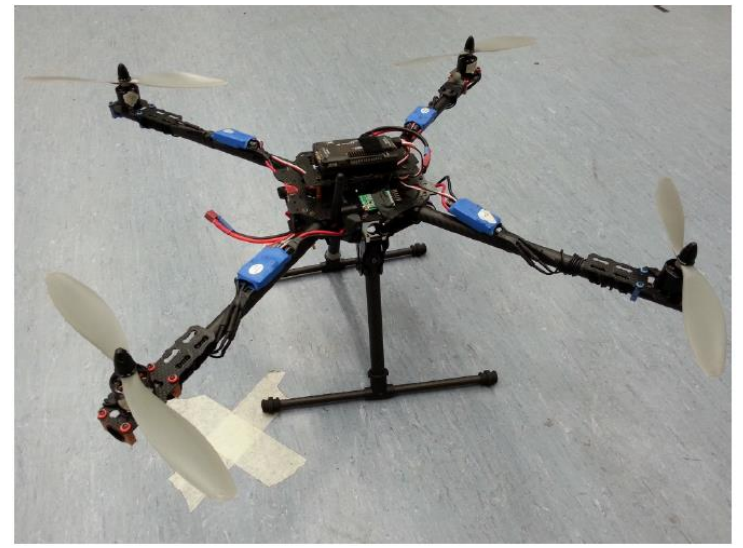
\includegraphics[scale=0.8]{images/Cuong-Quadcopter.png}
	        		\caption{Một Quadcopter}
	        	\end{center}
        \end{figure}
        
    	\subsection{Linh kiện điện tử}
Các linh kiện điển tử sử dụng được tóm tắt qua bảng sau:
\begin{tabular}{|c|c|c|}
\hline 
Số lượng & Tên & Trọng lượng \\ 
\hline 
4 & Bộ điều tốc & 32g \\ 
\hline 
4 & Động cơ không chổi than & 55g \\ 
\hline 
1 & Pin Li-Po & 250g \\ 
\hline 
4 & Phích cắm & 1g \\ 
\hline 
1 & Bộ chuyển đổi 4 ra 1 & 3g \\ 
\hline 
1 & Bộ chuyển đổi điện áp & 3g \\ 
\hline 
1 & AdruPilot Mega 2.5 & 31g \\ 
\hline 
1 & Bộ thu tín hiệu & 9.4g \\ 
\hline 
\end{tabular} 

\begin{itemize}
\item Bộ điều tốc được sử dụng được thiết kế riêng cho động cơ có nhiều Rotor. Mỗi bộ điều tốc nặng 32 gam với kích thước 55mmx26mmx11.6mm (rộng, dài, cao). Bộ điều tốc cung cấp năng lượng cho Motor và kiểm soát tốc độ quay của Rotor. Bộ điều tốc này cũng có chức năng giảm điện áp khi Quadcopter hoạt động ở công suất thấp.
\begin{figure}[h!]
	        	\begin{center}
	        		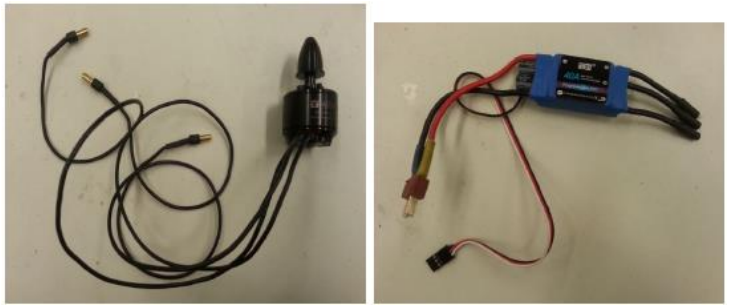
\includegraphics[scale=0.8]{images/Cuong-ESC.png}
	        		\caption{Bộ điều tốc}
	        	\end{center}
        \end{figure}
\item Các động cơ được sử dụng là động cơ không chổi than. Mỗi động cơ nặng 55gam (có thể lên tới 800gam tùy vào cánh quạt sử dụng) và có kích thước 27.5mm x 28mm (dài, cao).

\item Pin được sử dụng là pin Li-Po. Nó có điện áp 11.1V và dung lượng pin là 3300mAH. Dung lượng pin càng lớn thì thời gian sử dụng càng nhiều. Do ta đang sử dụng 4 motor nên ta phải dùng pin có năng lượng đủ lớn. Tuy nhiên nếu pin có dung lượng càng lớn thì kích thước và trọng lượng càng tăng. Trong Quadcopter này, ta dùng pin nặng 250gam và có kích thước 43mm x 130mm x 13mm (rộng, dài, cao). Quad-Rotor có thể bay trong vòng 10 – 15 phút với loại pin Li-po này.
\begin{figure}[h!]
	        	\begin{center}
	        		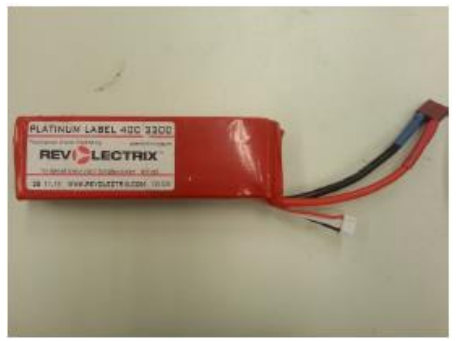
\includegraphics[scale=0.8]{images/Cuong-Battery.png}
	        		\caption{Pin Li-po}
	        	\end{center}
        \end{figure}
\item Các phích cắm được hàn với bộ điều tốc để nối với pin qua lỗ cắm. Nó có thể cho dòng điện có cường độ 40A chạy qua. Ta cũng có thể dễ dàng cắm, rút phích vào/ra lỗ cắm.

\item Bộ chuyển đổi gồm 4 lỗ cắm ra 1 phích cắm. Phích cắm của bộ điều tốc sẽ cắm vào 4 lỗ cắm của bộ chuyển đổi. Phích cắm của bộ chuyển đổi sẽ nối với pin. Chỉ cần 1 bộ chuyển đổi là có thể cấp năng lượng cho 4 bộ điều tốc từ 1 viên pin.

\item Bộ chuyển đổi điện áp có đầu ra là 6 cổng cung cấp điện áp 5.3V và dòng điện 2.25 A. Ta sử dụng bộ chuyển đổi điện áp để cấp nguồn cho ArduPilot Mega. Bộ chuyển đổi chấp nhận nguồn vào lên đến 18V và 90A.
\begin{figure}[h!]
	        	\begin{center}
	        		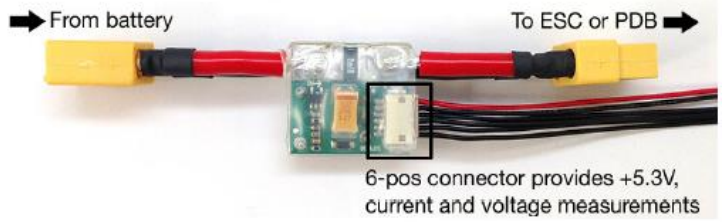
\includegraphics[scale=0.8]{images/Cuong-PowerModule.png}
	        		\caption{Bộ chuyển nguồn}
	        	\end{center}
        \end{figure}
\item ArduPilot Mega 2.5 là một trình điểu khiển hệ thống mã nguồn mở. Phiên bản Ardupilot này có thiết kế PnP, không cần phải lập trình. Tuy nhiên, nó cũng cho phép người dùng lập trình bằng phần mềm Arduino. Chức năng của thiết bị này là biến các phương tiện như xe, thuyền, máy bay thành các phương tiện không người lái.
\begin{figure}[h!]
	        	\begin{center}
	        		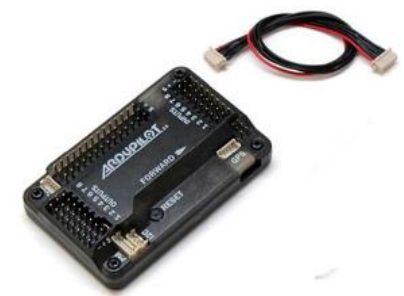
\includegraphics[scale=0.8]{images/Cuong-Adrupilot.png}
	        		\caption{AdruPilot Mega 2.5}
	        	\end{center}
        \end{figure}
\item Ta sử dụng bộ thu tín hiệu 8 kênh có tần số 2.4GHz. Nó được kết nối với vệ tinh. AR 8000 hoạt động trên tần số vô tuyến, nó có thể thấy được sự thay đổi của tín hiệu ngoài môi trường. Tín hiệu từ bộ thu sẽ được xử lý bằng phần mềm Spektrum để tạo thành “hình ảnh” sinh động nhất của tín hiệu vô tuyến. Sử dụng tần số 2.4GHz sẽ giúp tín hiệu được truyền tải liên tục, không bị nhiễu bởi các tần số khác. Sau khi kết nối bộ thu - phát tín hiệu thì bộ thu – phát sẽ chỉ kết nối với nhau nên nó không bị các tín hiệu khác làm nhiễu.
\begin{figure}[h!]
	        	\begin{center}
	        		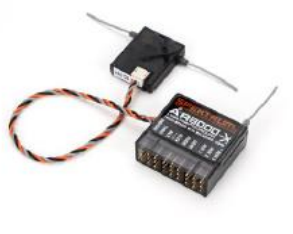
\includegraphics[scale=0.8]{images/Cuong-Receiver.png}
	        		\caption{Bộ thu tín hiệu}
	        	\end{center}
        \end{figure}
        \end{itemize}
    \section{Nguyên lý hoạt động}
    Một Quadcopter gồm 4 động cơ cánh quạt gắn với nhau. Khi động cơ quay, nó sẽ tạo ra lực nâng theo phương thẳng đứng.Cánh quạt quay càng nhanh thì lực nâng càng lớn và ngược lại. Vì thế, Quadcopter có thế bay lên cao hoặc hạ xuống thấp nhờ vào sự thay đổi tốc độ quay của các cánh quạt. Để Quad-rotor bay được thì tổng lực nâng tạo ra bởi 4 động cơ phải bằng hoặc lớn hơn lực hấp dẫn của Quadcopter.  
    Quadcopter có thể di chuyển theo phương ngang bằng cách thay đổi lực nâng của các cặp cánh quạt. Nếu tất cả các Rotors quay theo chiều kim đồng hồ, Quadcopter sẽ bị mất kiểm soát do phản lực của momen xoắn. Để tránh trường hợp trên thì ta sẽ cho cặp cánh phía trước (front) và cặp cánh phía sau (back) quay ngược chiều kim đồng hồ, trong khi đó cặp cánh bên phải (right) và bên trái (left) lại quay cùng chiều kim đồng hồ để triệt tiêu các momen xoắn.
    \begin{figure}[h!]
	        	\begin{center}
	        		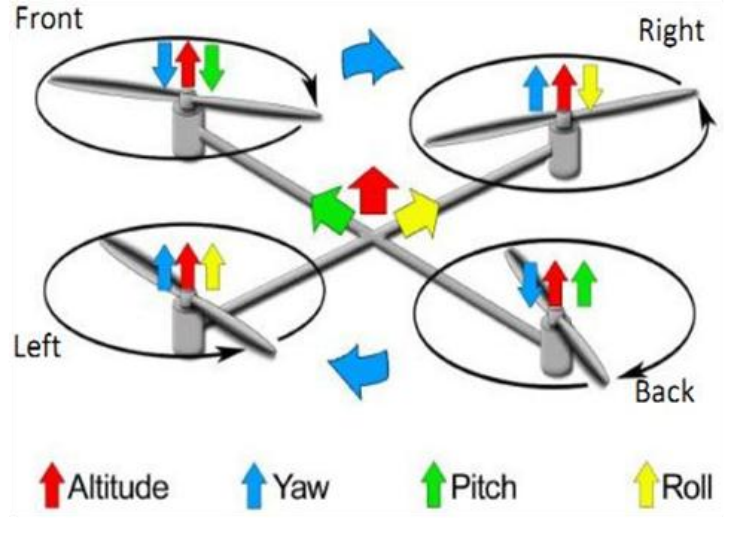
\includegraphics[scale=0.8]{images/Cuong-MoveSim.png}
	        		\caption{Chuyển động cơ bản của QuadCopter}
	        	\end{center}
        \end{figure}
        \subsection{Hệ quy chiếu}
Quadcopter được mô hình hóa theo hệ tọa độ tham chiếu Trái Đất Phẳng. Hệ toạ độ tham chiếu Trái Đất Phẳng bỏ qua lực ly tâm và gia tốc Coriolis.
Khung tham chiếu gồm các trục tọa độ (x, y, z) là hệ thống các trục đơn giản được dùng để xác định số lượng hoặc độ lớn. Hệ trục này có thể được gắn vào thân của vật hoặc Trái Đất. Trong trường hợp này, các trục của vật (xb,yb,zb) đang quay với trọng tâm là Quad-Rotor và các trục Trái Đất (xe, ye, ze) được biểu diễn như hình.                     
        \subsection{Mô hình động lực học}
        Nguyên lý hoạt động chính của mô hình này hoạt động dựa trên sự chuyển động của các dòng khí do cánh máy bay tạo ra và sự điều chỉnh vận tốc quay của cánh quạt sẽ làm thay đổi hướng bay của Quadcopter.
        \\
        Để mô tả chuyển động của Quadcopter ta cần 2 hệ quy chiếu:
        \begin{itemize}
        \item e_1 hệ quy chiếu Trái Đất.
        \item e_B hệ quy chiếu khung Quadcopter.
        \end{itemize}
        \\
        \begin{figure}[h!]
	        	\begin{center}
	        		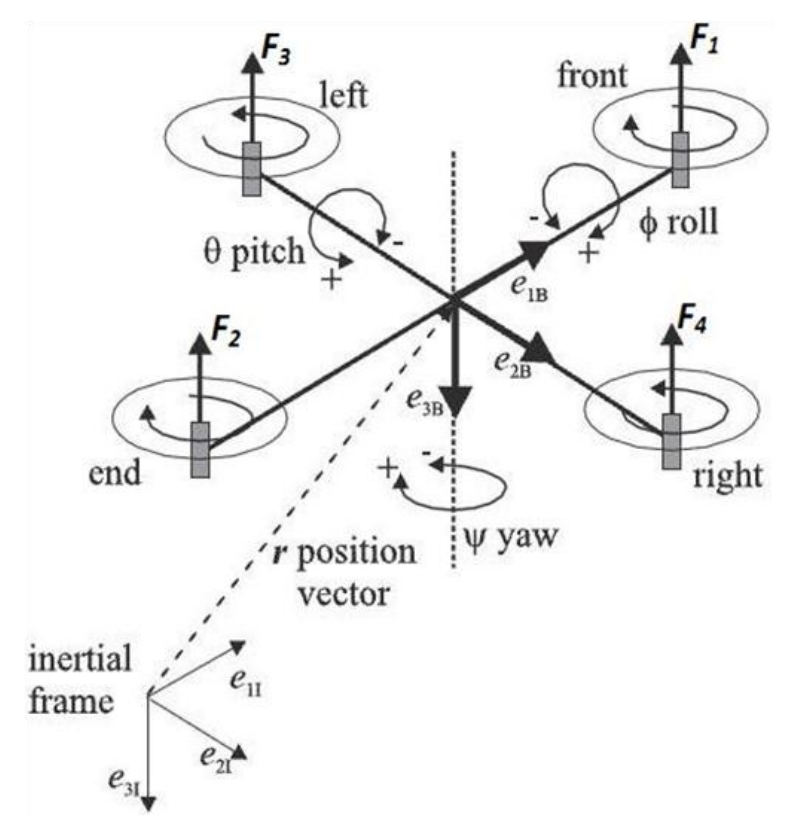
\includegraphics[scale=0.8]{images/Cuong-reference.png}
	        		\caption{Hệ quy chiếu A và B với chiều dài 1 trục L, tổng khối lượng mô hình m}
	        	\end{center}
        \end{figure}
        Sự định hướng Quadcopter được biểu thị bởi 3 góc Euler qua ma trận xoay R(1)
        \\
        \begin{figure}[h!]
	        	\begin{center}
	        		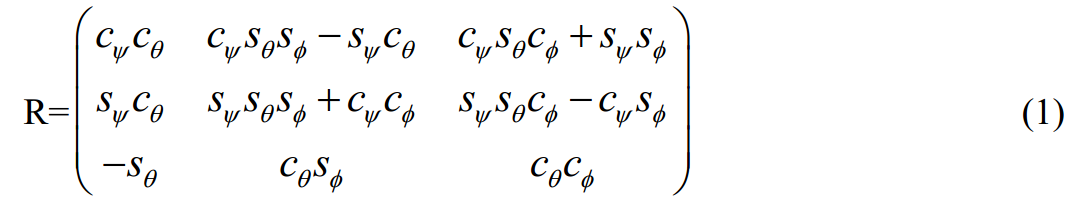
\includegraphics[scale=0.8]{images/Cuong-R1.png}
	        	\end{center}
        \end{figure}
        Lực sinh ra của các rotors: F_i = b.\omega_i^2, i = 1, 2, 3, 4
       \\
        Khi đó lực nâng cho cả khung máy bay là:
        \\
        \begin{figure}[h!]
	        	\begin{center}
	        		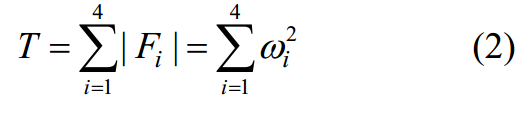
\includegraphics[scale=0.8]{images/Cuong-2.png}
	        	\end{center}
        \end{figure}
        Phương trình mô tả gia tốc Quadcopter:
        \\
        \begin{figure}[h!]
	        	\begin{center}
	        		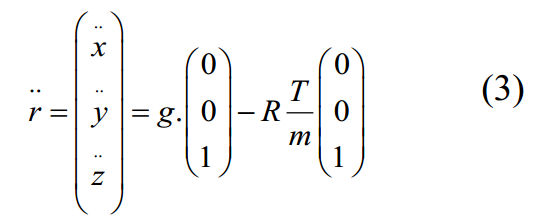
\includegraphics[scale=0.8]{images/Cuong-3.png}
	        	\end{center}
        \end{figure}
        Phương trình quan hệ giữa ma trận quán tính I_R = (I_x, I_y, I_z), momen quay M và momen quay hồi chuyển:
        \\
        \begin{figure}[h!]
	        	\begin{center}
	        		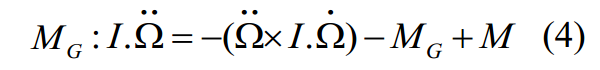
\includegraphics[scale=0.8]{images/Cuong-4.png}
	        	\end{center}
        \end{figure}
        Ta có momen quay hồi chuyển phụ thuộc vào các yếu tố vận tốc xoay với u_1 = T, u_2, u_3, u_4 lần lượt là các đơn vị momen quay các chuyển động roll, pitch, yaw hay vận tốc quay u^T=(u_1, u_2, u_3, u_4) và vận tốc góc \omega_i máy bay sẽ được g(u) = w_1 + w_2 - w_3 - w_4 (5)
        \\
        Kết hợp (5) với (3) và (4) ta có phương trình động lực học: (6)
        \begin{figure}[h!]
	        	\begin{center}
	        		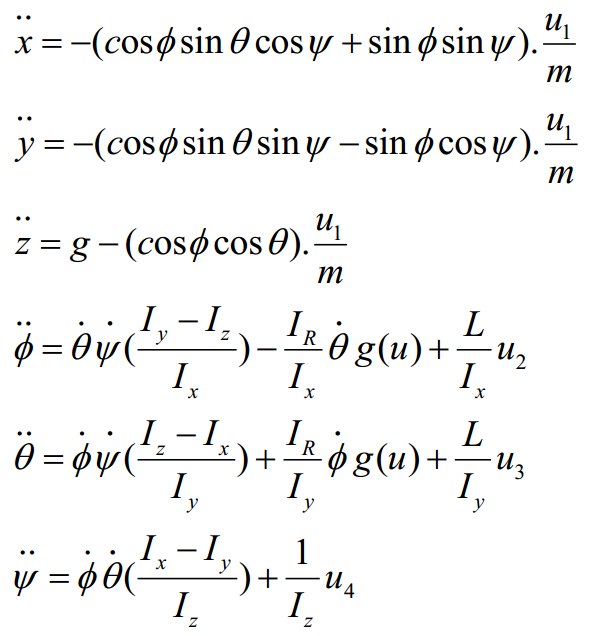
\includegraphics[scale=0.8]{images/Cuong-6.png}
	        	\end{center}
        \end{figure} 
        \subsection{Mô hình tính toán khí động học}
        Việc tính toán khí động học mô tả các tác động khi quay của cánh quạt trong không khí. Với các thông số T_{MT(N) là lực đẩy của cánh quạt, hướng lên, S(m^2) là diện tích của cánh quạt, ps (kg/m^3) là mật độ không khí
        \\
        Ta có phương trình lực đẩy:
        \\
        T_{MT} = 2p_sSv_1^2(N)
        \\
        Do lực đẩy T_{MT} = W_p = mg/4 (trọng lượng được mang bởi 1 cánh quạt):
        \\
        Vận tốc dòng khí cho mỗi cánh quạt V_1 = \sqrt{(W_p)/(2p_sS)} (m/s) 
     \section{Bộ điều khiển bay Quadcopter}
     \subsection{Thiết kế bộ điều khiển bay}
            Bộ điều khiển phải đảm bảo rằng Quadcopter phải đáp ứng được các yêu cầu đầu vào một cách chính xác nhất. Một cấu trúc kiểm soát vòng lặp kín được sử dụng trong bộ điều khiển này vì nó sẽ làm giảm sự xáo trộn và thích nghi nhanh với bất kỳ thay đổi nào trong quá trình bay của Quadcopter. Sự phân bố trọng lượng không đều của Quadcopter cũng có thể giải quyết bằng vòng lặp kín.
            \\
            \begin{figure}[h!]
	        	\begin{center}
	        		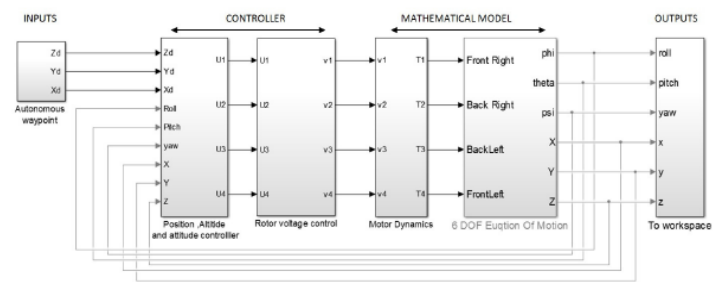
\includegraphics[scale=0.8]{images/Cuong-ModelofQc.png}
	        		\caption{Mô hình điều khiển Quadcopter}
	        	\end{center}
        \end{figure}
            Bộ điều khiển vòng lặp kín phải đảm bảo output phải sát với input. Vòng lặp điều khiển kín là nghịch đảo của động lực Quad-Rotor. Khi biết được động lực của Quad-Rotor, bộ điều khiển sẽ được điều chỉnh và nghịch đảo của động lực Quad-Rotor sẽ được tính. Kết quả tín hiệu điều khiển "U" được đưa vào mô hình để cho ra output mong muốn.
            \begin{figure}[h!]
	        	\begin{center}
	        		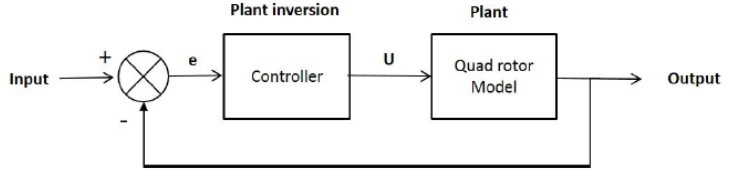
\includegraphics[scale=0.8]{images/Cuong-ClosedLoopControl.png}
	        		\caption{Mô hình điều khiển vòng lặp kín}
	        	\end{center}
        \end{figure} 
            \subsection{Nguyên lý hoạt động}
            Bộ điều khiển được xây dựng với các vòng lặp PD. Các vòng lặp PD sẽ có trong các hành vi, độ cao và vị trí của Quad-Rotor để tạo ra tín hiệu điều khiển tương ứng. Quad-Rotor sẽ sử dụng hệ thống điều khiển PD để xác định thời gian phản hồi và giải quyết yêu cầu của nó. Bộ điều khiển PD là một hệ thống phản hồi vòng lặp kín mà nó sẽ dùng output của tín hiệu điều khiển và gửi nó vào tín hiệu input ban đầu. Ta sẽ tính toán được sự khác nhau giữa hai tín hiệu và đưa ra sự điều chỉnh. Trong trường hợp này, vị trí và hướng của Quad-Rotor hiện tại (tín hiệu output) sẽ được gửi đến và so sánh với vị trí và hướng mong muốn (tín hiệu input) để cho phép hệ thống điều chỉnh input và các quá trình tương ứng.
\\
			Tín hiệu sai số được thể hiện bằng công thức: e(t) = r(t) - y(t)
\\
			Trong đó, e(t) là tín hiệu sai số, r(t) là tín hiệu input, y(t) là tín hiệu output.
			\begin{itemize}
			\item "Điều khiển tỷ lệ" là thuật ngữ phụ thuộc vào sai số điều khiển. Nó có thể kiểm soát bất cứ phần ổn định nào. Tăng tính cân đối sẽ làm giảm thời gian phản hồi của hệ thống điều khiển. Tuy nhiên, nếu tăng tính cân đối quá cao thì hệ thống sẽ không ổn định. Phương trình cân đối: u(t) = K_p e(t)
\\
Trong đó, u(t) là tín hiệu input trong Quad-Rotor, e(t) là tín hiệu lỗi, kp là gia lượng tỷ lệ.
			\item Điều khiển dẫn xuất là khái niệm output giảm khi các biến quá trình đang tăng. Nó tác động lên tỷ lệ thay đổi lỗi. Tăng điều khiển dẫn xuất sẽ làm cho hệ thống phản hồi mạnh mẽ với các thay đổi của lỗi và tăng tốc độ phản hồi.
			\\
			u(t) = K_dd[e(t)]/dt
			\\
			Trong đó, Kd là hệ số đạo hàm
			\item Để xác định được giá trị của Kp và Kd, ta phải điều chỉnh bộ điều khiển cho đến khi đạt được  phản hồi mong muốn. Ta dùng phương pháp Ziegler-Nichols và thủ công (trong hầu hết các trường hợp) để điều chỉnh các tỷ lệ và giá trị phái sinh. Ngoài ra, ta có thể dùng Simulink để điều chỉnh các giá trị tự động nhưng vẫn đáp ứng được yêu cầu của phản hồi.
			\end{itemize}
			\subsection{Cấu trúc bộ điều khiển}
			\begin{figure}[h!]
	        	\begin{center}
	        		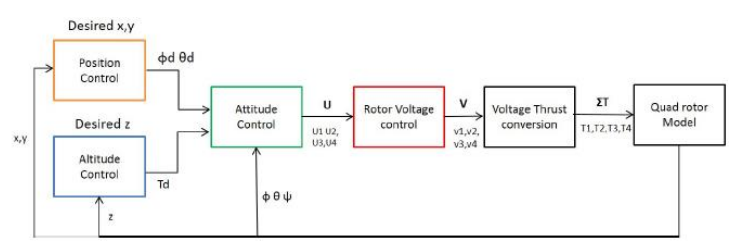
\includegraphics[scale=0.8]{images/Cuong-ControlArchitecture.png}
	        		\caption{Kiến trúc điều khiển}
	        	\end{center}
        \end{figure}
			Các góc Roll, Pitch, Yaw được điều khiển bởi các vòng lập PD bên trong, trong khi độ cao và vị trí được kiểm soát bởi các vòng lặp PD bên ngoài. Các vòng lặp ngoài sẽ tạo ta các giá trị mong muốn cho vòng lặp bên trong. Ta sẽ tập trung vào từng khối chi tiết trong phần sau.
\\
			\begin{itemize}
			\item Kiểm soát hành vi
			\begin{figure}[h!]
	        	\begin{center}
	        		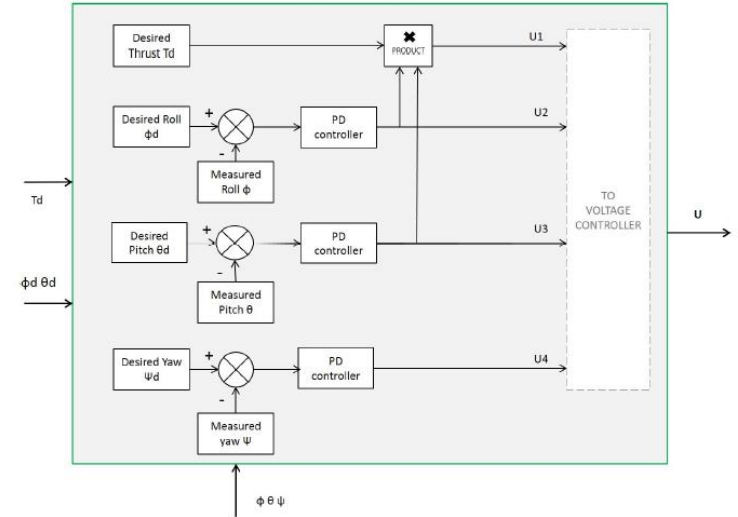
\includegraphics[scale=0.8]{images/Cuong-InnerloopIntiCon.png}
	        		\caption{Vòng lặp trong soát hành vi}
	        	\end{center}
        \end{figure}
			\\Vòng lập bên trong kiểm soát các góc Roll, Pitch và Yaw. Giả sử các trục x,y của Quad-Rotor đối xứng, tức là điều khiển góc Pitch và Roll giống nhau. Góc Pitch giảm khi di chuyển Quad-Rotor về phía trước dọc theo trục X trong khi góc Roll thì di chuyển Quad-Rotor về bên hông.
ROLL: Tín hiệu điều khiển U2 được tạo ra từ roller hoặc được truyền vào thông qua bộ điều khiển PD. Tín hiệu này sẽ điều chỉnh góc Roll của Quad-Rotor.
PITCH: Tín hiệu điều khiển U3 được tạo ra từ pitcher hoặc được truyền vào thông qua bộ điều khiển aPD. Tín hiệu này sẽ điều chỉnh độ cao của Quad-Rotor. Như đã nói ở trên giá trị của P và D của góc Roll và Pitch là như nhau.
YAW: Tín hiệu điều khiển U4 được tạo ra từ yawer hoặc được truyền vào thông qua bộ điều khiển PD. Tín hiệu này sẽ điều khiển góc YAW của Quad-Rotor. Giá trị của các góc Pitch, Roll, Yaw được đo sẽ là giá trị được nạp từ output của mẫu thử.
\\
			\item Kiểm soát độ cao
			\\
			Điều khiển vòng lặp ngoài này sẽ tạo ra một lực đẩy Td để nâng Quad-Rotor lên độ cao mong muốn. Nó được nạp thông qua bộ điều khiển PD. Td sau đó được chuyển đến bộ điều khiển độ cao để bù trừ cho hao hụt do vector của góc Pitch và Roll. Do đó, tín hiệu điều khiển U1 sẽ giữ được độ cao mong muốn của Quad-Rotor mà ngay cả khi góc Roll và Pitch thay đổi. Các khối điều khiển sau sẽ cho thấy vòng điều lặp điều khiển và tín hiệu tương ứng bên trong bộ điều khiển độ cao. Phản hồi nhận được cung cấp độ cao của Quad-Rotor.
\\
\begin{figure}[h!]
	        	\begin{center}
	        		\includegraphics[scale=0.8]{images/Cuong-OutterLoop.png}
	        		\caption{Vòng lặp ngoài kiểm soát độ cao}
	        	\end{center}
        \end{figure}
			\item Kiểm soát vị trí
			\\
			
		Vòng lặp ngoài này sẽ tính toán các góc roll và pitch để đưa Quad-Rotor đến vị trí X và Y mong muốn. Dữ liệu phản hồi từ mô hình cung cấp giá trị X và Y. Tín hiệu vị trí sau khi tổng hợp được nạp thông qua một bộ điều khiển PD và nó tạo ra các góc Roll và Pitch mong muốn. Như đã đề cập trước đó, output của nó sẽ được nạp vào bộ điều khiển hành vi để tạo ra các tín hiệu điều khiển U2 và U3.
\\
\begin{figure}[h!]
	        	\begin{center}
	        		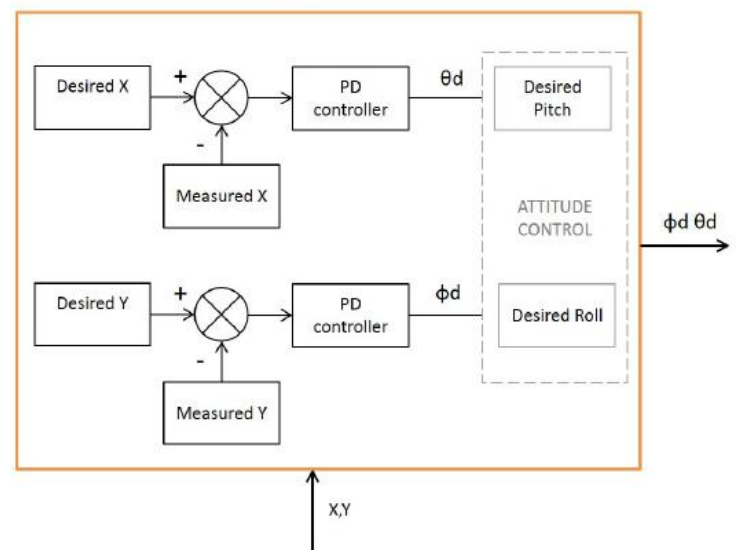
\includegraphics[scale=0.8]{images/Cuong-OuterLoopPos.png}
	        		\caption{Vòng lặp ngoài kiểm soát vị trí}
	        	\end{center}
        \end{figure}
			\item Kiểm soát điện áp của các Rotors
			\\
			Bốn inputs điều khiển được tạo ra bởi các vòng lặp trong và ngoài, nó không nạp trực tiếp vào mô hình Quad-Rotor vì nó là inputs lực đẩy cho bốn động cơ cánh quạt. Các tín hiệu điều khiển U được kết hợp để tạo ra tín hiệu điện áp cho mỗi Rotor. Sự kết hợp này dựa vào lực của Quad-Rotor để hiển thị thông số bay tương ứng. Sự kết hợp này đã được nói ở phần động cơ Rotor và được hiển thị như sơ đồ khối bên dưới. Điện áp đầu ra V sau đó được chuyển thành lực đẩy động cơ của mô hình.
  \\
  \begin{figure}[h!]
	        	\begin{center}
	        		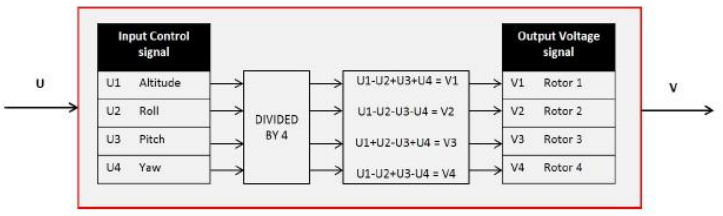
\includegraphics[scale=0.8]{images/Cuong-VolControl.png}
	        		\caption{Kiểm soát điện áp Rotors}
	        	\end{center}
        \end{figure}
			\end{itemize}
            Sau đó, Bluetooth Mesh dùng cơ chế publish-subscribe để các gói tin tới được nơi cần tới. Các địa chỉ unicast được đánh cho các element trong node và được gọi là publish address, còn có multicast address và vitural address bao gồm nhiều element (địa chỉ multicast thường đại diện cho cho một tầng lầu, một phòng,... trong thực tế). Khi có tin mới được gửi đến một địa chỉ publish address, bất kỳ những model nào (element bao gồm nhiều model) trong element và có đăng ký nhận tin (subscribe) ở địa chỉ đó sẽ nhận được tin.
        
            \begin{figure}[h!]
        	    \begin{center}
        		    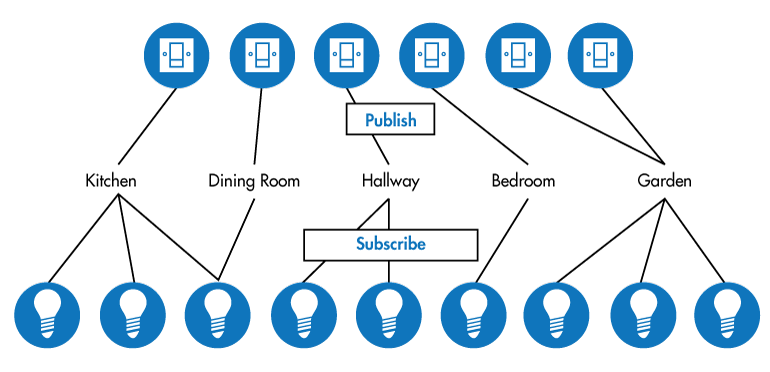
\includegraphics[scale=0.5]{images/mesh-pub-sub.png}
        		    \caption{Sơ đồ của cơ chế publish-subscribe}
        	    \end{center}
            \end{figure}